\documentclass[a4paper]{report}
\usepackage{setspace}
%\usepackage{subfigure}

\pagestyle{plain}
\usepackage{amssymb,graphicx,color}
\usepackage{amsfonts}
\usepackage{latexsym}
\usepackage{amsmath}
\usepackage[a4paper, margin = 3cm, bottom = 2.5cm]{geometry}
\usepackage{wrapfig}

\newtheorem{theorem}{THEOREM}
\newtheorem{lemma}[theorem]{LEMMA}
\newtheorem{corollary}[theorem]{COROLLARY}
\newtheorem{proposition}[theorem]{PROPOSITION}
\newtheorem{remark}[theorem]{REMARK}
\newtheorem{definition}[theorem]{DEFINITION}
\newtheorem{fact}[theorem]{FACT}

\newtheorem{problem}[theorem]{PROBLEM}
\newtheorem{exercise}[theorem]{EXERCISE}
\def \set#1{\{#1\} }

\newenvironment{proof}{
PROOF:
\begin{quotation}}{
$\Box$ \end{quotation}}



\newcommand{\nats}{\mbox{\( \mathbb N \)}}
\newcommand{\rat}{\mbox{\(\mathbb Q\)}}
\newcommand{\rats}{\mbox{\(\mathbb Q\)}}
\newcommand{\reals}{\mbox{\(\mathbb R\)}}
\newcommand{\ints}{\mbox{\(\mathbb Z\)}}

%%%%%%%%%%%%%%%%%%%%%%%%%%


\title{{\vspace{-14em} 
\includegraphics[scale=0.4]{ucl_logo.png}}\\
{{\Huge 3D model construction from 2D images}}\\
{\large Visual Hull in Python 3}\\
}
\date{Submission date: Day Month Year}
\author{Khwaja Yasir Muzib\thanks{
{\bf Disclaimer:}
This report is submitted as part requirement for the MY DEGREE at UCL. It is
substantially the result of my own work except where explicitly indicated in the text.
\emph{Either:} The report may be freely copied and distributed provided the source is explicitly acknowledged
\newline  %% \\ messes it up
\emph{Or:}\newline
The report will be distributed to the internal and external examiners, but thereafter may not be copied or distributed except with permission from the author.}
\\ \\
Computer Science\\ \\
Supervisor's name: Dariush Hosseini \\
Supervisor's name: Tobias Ritschel}



\begin{document}
 
\onehalfspacing
\maketitle
\begin{abstract}
This project aims to solve construction of a 3-dimensional model in a virtual space from plain images. As input, we have captured plain images of an object  from different angles and orientations by putting the object on a rotating table. For the different orientations the precise co-ordinates and angles are noted. Then  we intend to use these images as the dataset to create a 3D model of that object using python. Having no experience of programming in python properly before and even more so of having no experience with 3D programming or Computer Vision principles before, I took this task as a challenge to teach myself all these skills to be able to do this project. I start out with reading papers as to how 3D construction has been done and then worked on a code file to explore and understand these concepts to greater detail.
\end{abstract}
\tableofcontents
\setcounter{page}{1}


\chapter{Introduction}
Virtual World is a fascinating and upcoming latest state of the art technology.
A lot more is represented and a much more imaginative world than our real human-world can be viewed and experienced virtually through this technology. My work focuses on the very core aspect of this. That is translating the real world to a virtual space.
\\
Definition:
\begin{center}
A virtual  space is a computer-simulated environment that mimics the real world. There are no topographical or geographical limits in this world.
\end{center}

\section{Motivation}
The biggest motivation for me is from video games. The entirety of the gaming world is based in a virtual world. However its application are not limited to games, but to medical imaging, geographical mapping, human face detection and  object detection are a few.
\begin{figure}[h]
{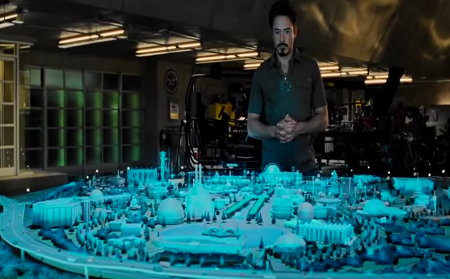
\includegraphics[scale=1]{ironmanmap.jpg}}
\caption{Iron Man Hologram Scene}
\end{figure}
\\
However to mention the single scene that got me into thinking about Computer Vision and its might is this part from Iron Man where it showcases a hologram of map buildings. That is what got me into thinking what if I take pictures of all the buildings in the world (thankfully already available through Google Maps) and then make a program to simulate them in the virtual space just like this scene.
\newpage
\subsection{Augmented Reality}
\begin{wrapfigure}{O}{0.5\textwidth}
\centering
\includegraphics[scale=0.5]{pokemongo.jpg}
\caption{Pokemon Go}
\end{wrapfigure}
Augmented Reality is probably becoming one of the biggest technology trends of the modern time. With time it is going to be even bigger considering how smart-phone companies and game-console companies are trying to make devices that incorporate AR technology.
\\

AR can be characterized as a framework that satisfies three fundamental highlights: a blend of real and virtual universes, real-time interaction, and precise 3D registration of virtual and genuine objects. The smartphone app Pokemon Go, which was released in 2016 and soon became an inescapable phenomenon, is the most popular example of AR technology.
The sensory information overlaid on top can either be constructive (i.e., additive to the natural environment) or destructive (i.e. masking of the natural environment).
This experience is so well integrated with the physical world that it is considered as a fully immersive part of the real world. Augmented reality modifies one's ongoing experience of a real-world environment, while virtual reality fully replaces the user's real-world environment with a simulated one.
\\
In this how I visualize the Pokemon Go to be improved is if we had real models of buildings inside the game that would represent the buildings the player sees in real time, would be an excellent feature making the game more life-like.
\newpage

\subsection{3D  Object Recognition}
In a photograph or range scan, 3D object recognition entails recognizing and determining 3D details, such as the pose, length, or shape, of user-selected 3D objects. In most cases, a vision system is shown an image of the object to be identified in a controlled setting, and then the system locates the previously presented object with an arbitrary input, such as a video stream.
\\
The procedure for identifying a 3D structure is determined by the object's properties. This has been approached in two ways: 
\begin{center}
\begin{enumerate}
  \item pattern recognition 
  \item feature-based geometry.
\end{enumerate}
 \end{center} 
 Pattern recognition  approaches use low-level image presence knowledge to locate an object, and feature-based geometric approaches create a model for the object to be identified and align it against the picture. My study is more motivated towards  feature-based geometric approaches.

\subsubsection{Feature-based geometric approaches}
Feature-based methods are ideal for objects with distinct characteristics.
Feature-based object recognizers function by taking a specific set views of the object to be identified in advance, extracting features from these views, and then matching these features to the scene and applying geometric restrictions throughout the recognition process.
\\
\\
This very closely follows to the work that I intend to achieve in this project. According to the [Rothganger et al. 2004] which exemplifies this, the method creates a 3D model for the object based on a variety of camera views, which includes the 3D spatial location and orientation of each element. Since there are so many views of the object, each aspect is usually present in several adjacent views. Since the centre points of such matching features align, and observed features are oriented along the primary gradient direction, the points at (1, 0) in the feature parallelogram's local coordinate system, as well as the points (0, 1) in the parallelogram's local coordinates, indeed match. \\
Three point pair correspondences are thus known for any pair of matching features in neighboring views. Given at least two matching features, Structure From Motion Algorithm was used to make an estimate of the positions of the points.
\begin{figure}[h]
\includegraphics[scale=0.6]{roth_partial3d_features.jpg} 
\caption{Partially projected 3D projections of features created from surrounding views of a teddy bear. [Rothganger et al. 2004] }
\end{figure}
\newpage

\subsection{Remote Sensing}
Remote sensing involves gathering information about an object or phenomena without physically making any contact with the surface being surveyed. The concept of remote sensing mostly refers to gathering data about the Earth in particular and in recent case also about Mars.
\\
It is used in various fields, largely being used for land surveying. It has wide applications in military or economic planning, commercial development, deep-sea exploration. To record the information about surrounding, a pulse radar emits pulses of energy to scan for objects and locations, during which a sensor absorbs and analyses the reflected and scattered radiation from the target. Examples are The RADAR and LIDAR technology. These devices extrapolate the sensor data with respect to a reference point including distances among the already known points on the ground. 
\\
\subsubsection{LiDaR - Light Detection and Ranging}
This technology is now equipped with smartphones. Iphone 12 has a 3D scanning app, that lets users scan objects around them and put them in a AR world using LiDaR technology.
\begin{figure}[h]
\includegraphics[scale=0.15]{lidarApple.jpg} 
\caption{Making a furniture a model in our phones using LiDaR technology}
\end{figure}
The fact that this comes packaged  along with phones motivates me to work on this and take the application usage of this further. With this in hand, a user could scan around anything ranging from objects to buildings around them, and since long this has been used in submarines as well.
\\
\begin{wrapfigure}{r}{0.5\textwidth}
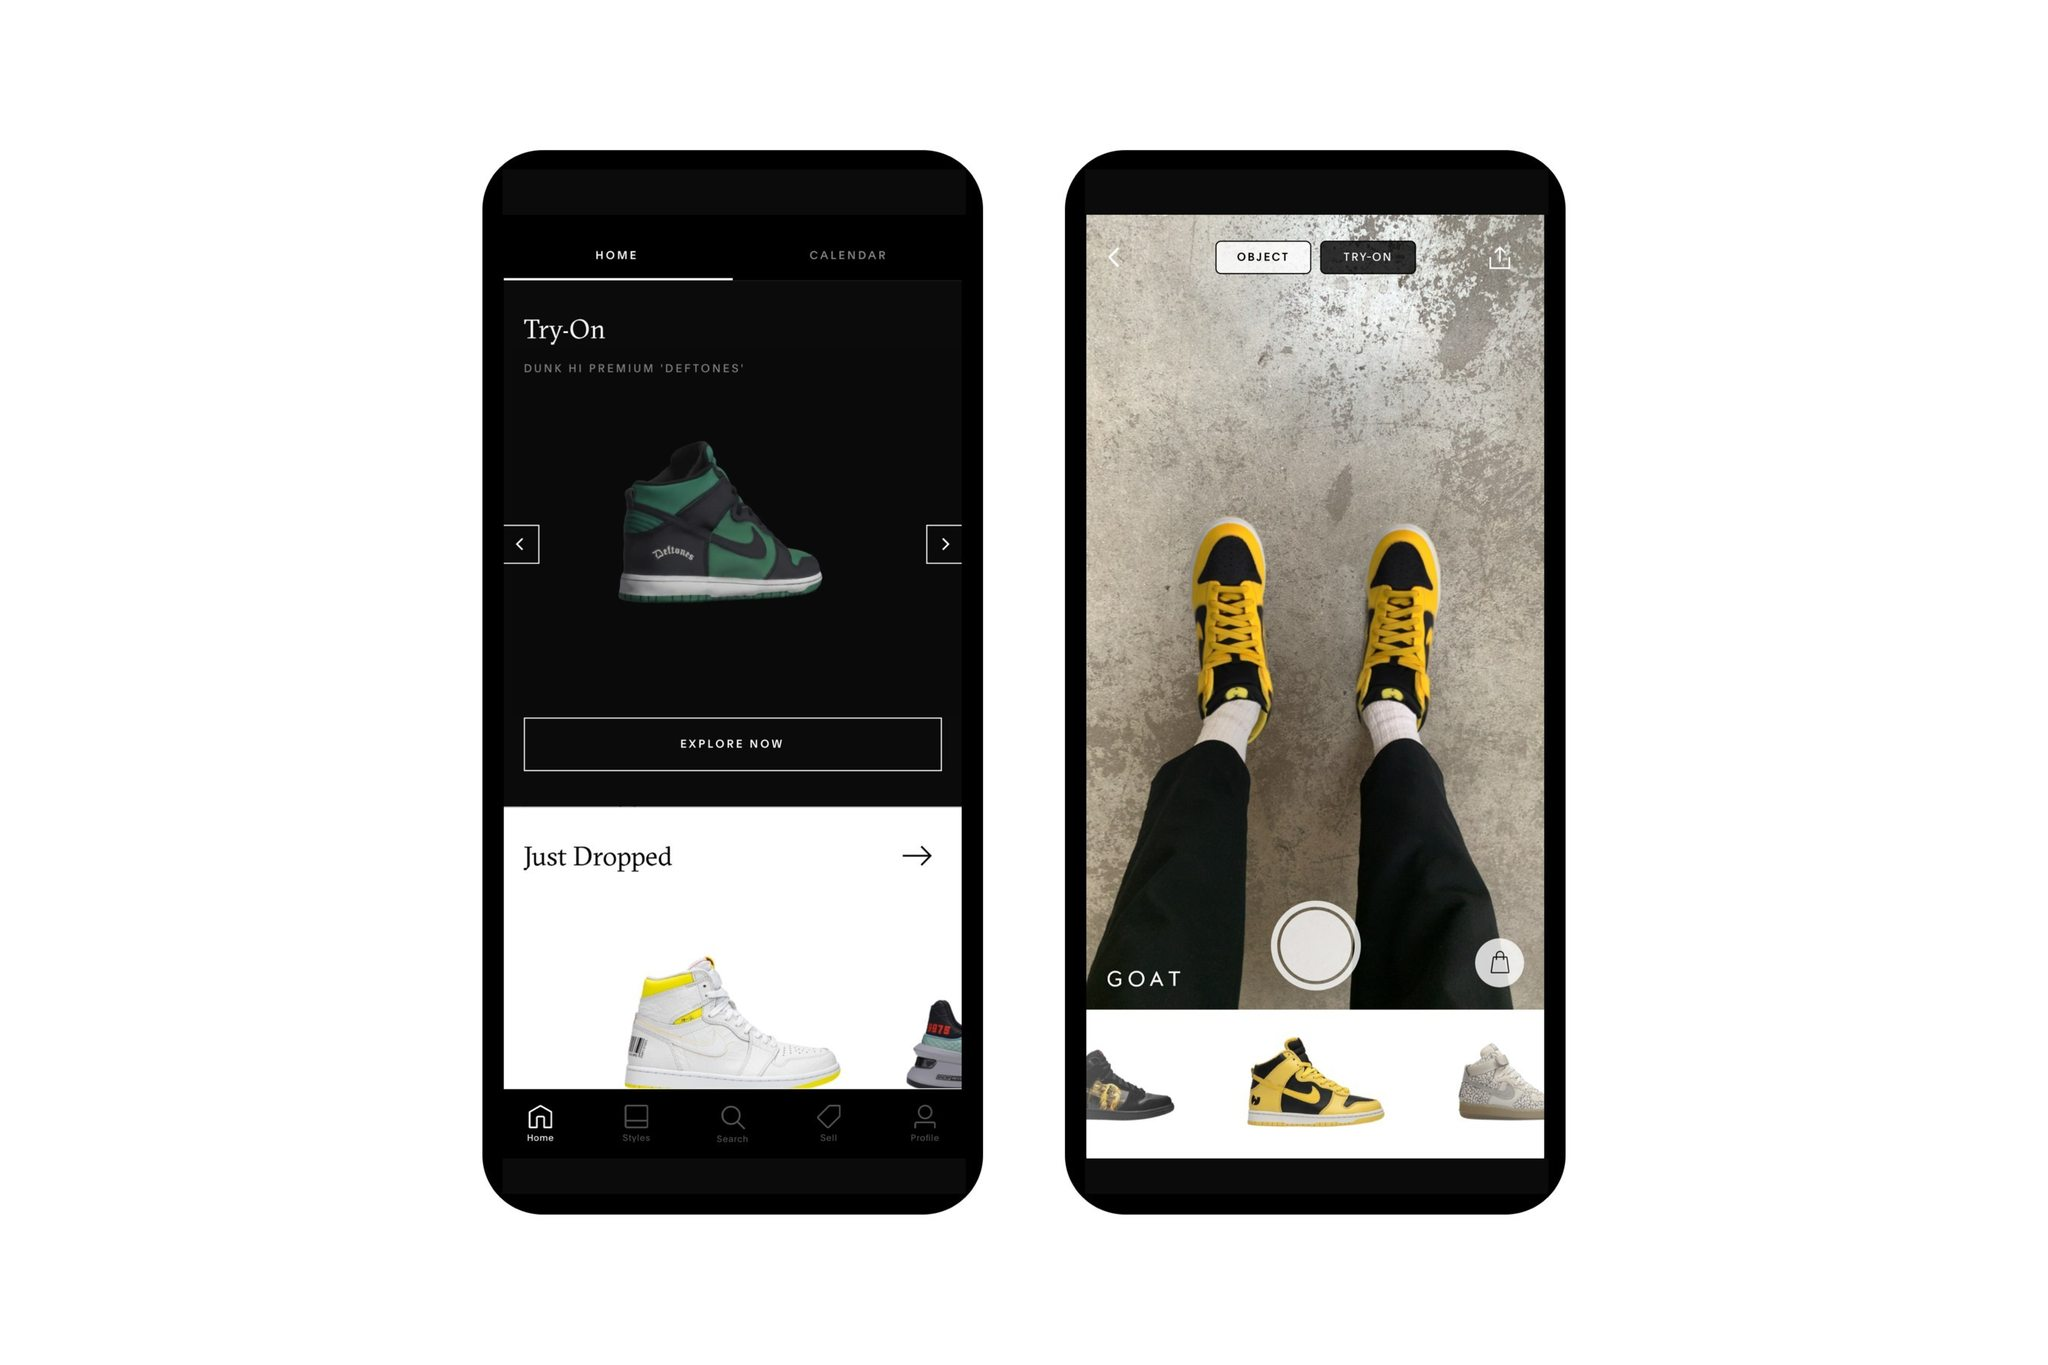
\includegraphics[scale=0.15]{GOAT.jpg} 
\end{wrapfigure}
\\
I could go around my building taking a scan of it, and then remodel it in an app. I could also take a scan of the entire interior and put it in Unity or Unreal Engine where I could do interior designing using custom made objects. 
\\

A recent trend, where shopkeepers use similar technology to measure the size of one's feet to recreate a customer wearing a shoe inside the app without the customer ever having to visit a shop. 
\newpage


\section{Project Objectives}
Mathematical expressions are placed inline between dollar signs, e.g. $\sqrt 2, \sum_{i=0}^nf(i)$, or in display mode
\[ e^{i\pi}=-1\] and another way, this time with labels,
\begin{align}
\label{line1} A=B\wedge B=C&\rightarrow A=C\\
&\rightarrow C=A\\
\intertext{note that}
n!&=\prod_{1\leq i\leq n}i \\
\int_{x=1}^y \frac 1 x \mathrm{d}x&=\log y
\end{align}
We can refer to labels like this \eqref{line1}.   

\chapter{Background Study and Literature Review}

For a computer vision project, the first steps to trace to is the methodology and the design decisions taken in order to implement it.The first step hence is by investigating the ways in which the 3D shape  is acquired.  From moons 2009 paper, we learn about the different available 3D acquisition categorizations.
\section{3D Acquisition}
For all the 3D capturing methods available, there is a distinction between active and passive methods. To obtain 3D data from active techniques, the light sources are carefully monitored. The light intensity in active lightning is moderated in some way, either perceptually or spatially. For passive methods, light is not regulated or is only controlled in terms of picture clarity, mostly uses whatever light is available in the environment that is ambient light.
\\
As our interest is in capturing information is in which no external measures are taken, such as adding illuminated lightning, since we want to keep our purpose as simple as using the program using  sensors equipped in our handheld devices such as smartphones, we are only interested in passive methods where we only work on the raw data without any manipulation.
\\
\begin{center}
\textbf{For Passive 3D shape Extraction:}
\begin{enumerate}
\item Singular View-Point Methods
 \begin{enumerate}
 \item Shape from texture
 \item Shape from Occlusion
 \item Shape from Focus
 \item Shape from Contour
 \end{enumerate}
 
 \item Multiple View-Point Methods
 \begin{enumerate}
 \item Passive Stereo
 \item Structure from Motion
 \item Shape from Silhouette

 \end{enumerate}
\end{enumerate}

\end{center}

\subsection{Single View-Point}

%https://hal.archives-ouvertes.fr/hal-01190112/document
Single View-point methods work by using a "single view". For example, the Shape from Focus technique which is also referred to as the Depth from Focus is based on the foundation of the depth of field. 3D acquisition of a scene with high occlusions is solved using this technique.
\begin{center}
"Occlusion" is described as "the result of one object/point in a three-dimensional space blocking the view of another object/point" resulting in missing point/series of points or object in one view.
\end{center}

It uses a stack of 2D images to create a depth map of a picture. This stack is created by adjusting the camera/object distance according to a set of steps, with each step requiring the acquisition of an image in order to search the scene.
\\
\subsection{Multiple View-Point - Triangulation}
As the name suggests, it uses multiple images/view-points. The theory of triangulation is used in many multi-vantage methods to obtain depth knowledge.
\begin{center}
Triangulation is a surveying technique that involves measuring the angles created by three survey control points in a triangle. The other lengths in the triangle are determined using trigonometry and the estimated length of just one side.
\end{center}
We will be working with many view-points that is a collection of images that is easily obtainable using smartphones, hence multiple  view-point methods are further investigated.
\subsection{Stereo}
Stereo is the term for such a configuration where we have two photographs that were shot at the same time but from different perspectives. Stereo-based 3D reconstruction works on the following principle: given two projections of the same point in the universe into two images, the intersection of the two projection rays is used to determine the point's 3D direction. This method is repeated many times to achieve the 3D shape and orientation of the objects in the scene. Since this uses triangulation, the ray equations and complete knowsledge of the cameras: parameters such as their relative positions and orientations are needed for this operation.
\\
\begin{figure}[h]
\includegraphics[scale=1]{3dstereo.jpg} 
\caption{Ray intersection}
\end{figure}
\newpage
\subsection{Structure  from Motion}
SfM varies from Stereo in the basis that, for passive stereo, the images had to be static, however for SfM the camera is actually in motion.

\begin{figure}[h]
\includegraphics[scale=0.65]{sfm.jpg} 
\caption{Structure from Motion from }
%[https://gsp.humboldt.edu/OLM/Courses/GSP_216_Online/lesson8-2/SfM.html]
\end{figure}


\subsection{Visual Hull - Shape from Silhouette}
The Visual Hull is a 3D reconstruction principle based on the Shape from Silhouette (SFS) methodology. The basic concept is to combine silhouettes from several images taken from different angles to create a 3D representation of an object. Separate camera views project both of these silhouettes as a cone, and the intersection of each of these cones is a representation of the actual object's form. In certain ways, the visual hull carves out areas of space where the object is not present.
\begin{figure}[h]
\includegraphics[scale=0.30]{vsh.jpg} 
\caption{ Visual Hull}

\end{figure}
\\
The first photo on the top left, shows a single projection of a singular visual cone of the tea-pot. For the next two images, two more view-points are taken and similarly two more visual cones are projected on the tea-pot silhouettes.
The intersection of these backprojections forms the object's visual hull.
As further views are taken, the visual hull achieves its true state, but cavities not seen in the silhouettes are not restored.
\newpage
\subsection{Advantages of Visual Hull}

\begin{enumerate}
\item The silhouette equation is easy to apply when we assume an enclosed environment with regulated/ambient conditions, such as static light and static cameras.
\item The SFS-algorithm is simple to implement, particularly when compared to other shape estimation techniques such as multi-baseline stereo.
\item The object is always contained within a visual  hull. The SFS construction provides an upper bound of the real object's shape in comparison to a lower bound, which is a major advantage for obstacle avoidance in robotics or navigation visibility analysis.
\end{enumerate}

\subsubsection{Algorithm that object is contained within the volume produced}

Assume that a collection of R reference views is used to display an initial 3D object. The silhouette \(s_r\) is present in each reference view \(r\), with the interior pixels hidden by the object. For view \(r\), all the rays that start at the image's viewpoint \(p_r\) and pass through these interior points on the image plane determine the cone-like volume \({vh}_r\) . The real object is guaranteed to be included in \({vh}_r\). This statement remains true for all \(r\), meaning that the object must be contained within the volume \( {{vh}_R} = {\cap_{r\in R}vh_{r} }\).
\newline

\begin{wrapfigure}{l}{0.5\textwidth}
\includegraphics[scale=0.35]{volbound.jpg} 
\caption{Figure taken
from Cheung, 2003 \cite{Cheung:2003}}
\label{fig:voxelgrid}
\end{wrapfigure}
Figure (a) shows four perspectives \(C^1\), \(C^2\), \(C^3\) and \(C^4\), each with a unique viewpoint on the target O and hence separate silhouettes \(S_1^1\),\(S_1^2\),\(S_1^3\), and \(S_1^4\).The projected silhouettes converge to shape the Visual Hull \(H_1\). The difference between an object's Visual Hull and its approximation is shown in Figure (b). We can see that the yellow region is the unwanted , or yet to carved out space remaining. As claimed earlier, if we take \(R \rightarrow \infty \), then \({vh}_R\) converges to a form known as the visual hull \(vh\) of the original geometry and contains all possible views. Since concave surface regions can never be separated from silhouette details alone, the visual hull is not guaranteed to be the same as the original object.
\clearpage
\newpage
\section{Further look into constructing Visual Hull}
\subsection{Volume Carving}
Volume carving is a technique for converting silhouette contours into visual hulls. Each camera takes a picture of a clear part of an object that can be used to make a contour. As projecting onto the image plane, this contour encloses a collection of pixels known as the object's silhouette. Volume carving uses the silhouettes of figures from various angles to ensure consistency.
Since we know the object is contained within the intersection of its visual cones, we begin by specifying a working volume inside which we know the object is located. 
\\
This volume is subdivided into small units known as voxels, creating a voxel grid. A cross-sectional view of this can be seen in the figure b of  Figure \ref{fig:voxelgrid}. Each voxel in the voxel grid is projected onto each of the views. A voxel in a vision is discarded if it is not contained by the silhouette. As a result, at the end of the volume carving algorithm, we are left with the voxels enclosed within the visual hull.

\subsection{Volume Based Approach}
Another method to obtain visual hulls is a volume based approach which is very fast and simple, where the  virtual space is made up of voxels \(v\). A cuboid of voxels is considered, so there are total of  \(v = 1 ..N^3\) voxels.
\\ 
An Algorithm from \cite{Schneider:2014} is given:
\begin{figure}[h]
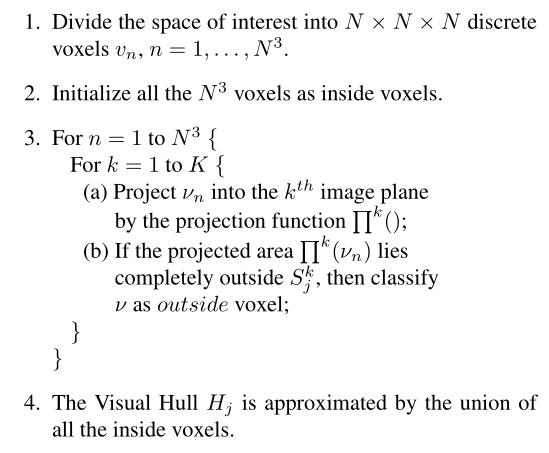
\includegraphics[scale=0.5]{volumeCarving.jpg} 
\end{figure}
\\
The final shape is depicted in this version by 3D volume voxels. The structure was then split into two parts, which we called inside and outside depending on whether they were in the visual cones.
\subsubsection{Disadvantage of volume based}
The resulting image is considerably greater than the actual object shape, it should only be used in applications where an approximation is used.[Cheung:03]
\newpage
\subsection{CSG Rendering}
Another method by which Visual Hulls are constructed is by the use of Constructive Solid Geometry rendering. Ray tracing can be used to render an object marked by a tree of CSG operations without explicitly computing the resulting solid \cite{Roth:82}. This is obtained by looking at each ray individually and computing the interval along the ray occupied by each object, again making use of the principle of intersection, in this case intersection of rays in 1D.
For each axis, a particular axis is chosen over which the CSG operations will then be carried out over the interval sets . The computation of a 3D ray-solid intersection is needed for this process. Due to the fixed cross section of the cone, 3D ray intersections can be simplified to 2D ray intersections.


\subsubsection{Calculation}
Each viewing ray's intersection with the visual hull is calculated given a desired view. Since computing a visual hull only requires intersection operations, the CSG calculations can be done in any order. Furthermore, in the sense of the visual hull, every CSG primitive is a projective visual cone.

\begin{figure}[h]
\includegraphics[scale=0.7]{rayInt.jpg} 
\caption{Ray Intersection}
\label{fig:rayInt}
\end{figure}
A scanline's pixels in the desired image trace a pencil of line segments in the reference image. An orderly scanline traversal can sweep out these segments such that their slope across the epipole differs linearly.
\\
\begin{center}
According to Figure\ref{fig:rayInt},

\end{center}\begin{enumerate}
\item On a reference image, a 3D viewing ray is projected.
\item The projected ray's intersection with the 2D silhouette is performed. These intersections result in a list of intervals around the ray that are interior to the cone's cross-section.
\item Each interval is then elevated back into 3D using a simple projective mapping and intersected with the results of the ray-cone intersections of other references.
\end{enumerate}
\subsubsection{Algorithm to compute by }
\begin{figure}[h]
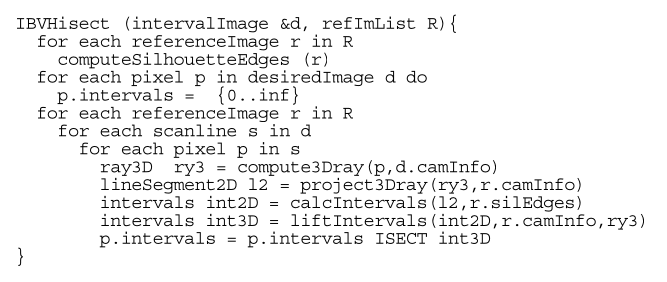
\includegraphics[scale=0.7]{intersection.jpg} 
\end{figure}
This is the algorithm to compute ray-intersection.
\begin{enumerate}
\item n is the number of pixels in a scanline
\item d is the number of pixels in an image
\item k is the number of references
\item l is the average of the intersection of the rays with silhouette
\end{enumerate}
The complexity of the running time for all the intersections for a desired view is \(O(lkn^3)\).
\subsection{Image Based}
In a paper from \cite{Chen:95},  they create 3D perspective viewing effects using real-time image processing. Cylindrical panoramas were used as the photographs. Since each image includes all of the details needed to look around in 360 degrees, the panoramas are orientation independent. A series of these images may be linked together to create a walkthrough chain.

A camera pointed at the object's center and orbiting in both the longitude and latitude directions in about 10-degree intervals is used to image it. This method generates hundreds of frames, one for each of the possible viewing directions. In dynamic playback, the frames are contained in a 2D sequence that is indexed by two rotational parameters.
\newpage

\section{Summary}
We have gone through how to acquire the 3D volume. We have looked at the methods in order to do this. We have also looked at some of the advantages regarding few methods  as to  how it can be beneficial to us, in terms of computational power, and also use case wise.
\\
Then we have further investigated the methods for constructing visual hulls.
We have gone through volume carving, volumetric approaches, CSG rendering and image based options.
\\
Most feasible for me to do, seemed to be the volume carving one. It is fast and efficient, has a much tighter convex hull around the object than volumetric approaches. And compared to CSG renderings and image based, it is much faster and simpler.
\\
On the other hand , even though image based visual hulls and CSG renderings do tend to produce much more accurate photo-consistent visual hulls, it is much more complex to implement, regarding that more work needs to be done on the algorithm to generate the ray-intersections and camera parameters.
\section{What we are trying to solve}
Firstly, I intend to take picture of an object and create a set for several views. Then this dataset is processed to make silhouettes.
Use these in order to create a matrix that holds the information of these images. Use these matrices to create
\newpage
\chapter{Modelling the Data}
Here we are mostly going to see the input dataset that we feed into our program to generate the visual hulls and later see how these input images are further processed for application usage.
\\
Dataset is produced and provided by Steve Seitz, James Diebel, Daniel Scharstein and Rick Szeliski of Univesity of Washington,
Stanford University, Middlebury College and Microsoft Research respectively.
\section{The raw datasets - Temple}
For our input, we take a toy temple as our input model.
16 images shown here to depict the orientation and different perspective views of our toy model. To make silhouettes, the background has been intentionally kept black in colour.
\\
These were taken after rotating the temple toy on a rotating table under ambient light focusing solely on the toy.
\begin{figure}[h]
\includegraphics[scale=0.46]{templeAll.jpg} 
\end{figure}
\newpage
\section{Silhouettes - Segmentation Methods}
Segmentation is the process of dividing an image into regions that correspond to objects. All pixels in the entire region of the image shares a common property. The intensity is the most basic property that pixels can share. 
\\
There are three different categories of segmentation methods are available:
\begin{enumerate}
\item Intensity-based segmentation - thresholding
\item Edge-based segmentation
\item Region-based segmentation
\end{enumerate}
Thresholding is basically the distinction between light and dark areas.
\\
Some assumptions are made about thresholding:
\begin{enumerate}
\item The different regions being classified have different intensity values
\item Among the individual regions, which represent a particular object or to say a common series of pixels have similar intensity values.
Example:
\end{enumerate}
\begin{figure}[h]
\includegraphics[scale=0.3]{threshold.jpg} 
\caption{Thresholding \cite{UoV:09}}

\end{figure}

\subsection{Intensity-based segmentation}
The process of separating one or more regions of significance in an image from regions that do not hold important information (in our case pixels) is known as segmentation. The fundamental premise for intensity-based strategies is that pixels belonging to features of interest have a different set of intensity values than the range of intensity values of  background pixels.
Background refers to regions that do not hold important information, such as in our case, that would be the black pixels in temple datasets. We also assume that background intensity values are lower than feature intensity values in our case.
\newpage

If we conclude that the distribution of feature pixels and background pixels is roughly Gaussian, we get a distinctive intensity distribution of two peaks in the histogram.
The distribution is bimodal, as we get two modes in total, one for the background and one for the feature.
\\
Because of the additive noise and intensity non-linearities of the features, intensities are usually distributed across the modal values. 
\\
The most basic solution to segmentation will be to use an acceptable intensity threshold. All pixels with values greater than the threshold value are classified as feature pixels, and all pixels with values less than the threshold value are classified as background pixels.
\\
This is displayed in the equation below:
\begin{equation}
I_T = 
\begin{cases} 
      1 & \textsf{for } I(x,y) \geq T\\
      0 & \textsf{for } I(x,y) < T
   \end{cases}
\end{equation}

This equation is used to create an image. In this image, according to the equation given, \( I(x,y)\) are the original image pixels, and \(I_T(x,y)\) are the image pixels after thresholding was done. It is known as a binary image since it contains only two values: 1 for feature pixels and 0 for background pixels.
\\
Since each location (x,y) of the original image has a value of 1 in the mask if it is a feature pixel, it can be used as a mask.

\begin{figure}[h]
\includegraphics[scale=1.5]{threshold_identifier.jpg} 
\caption{A Bimodal Histogram \cite{WWH}}
\label{fig:thresh}
\end{figure}

In general, background pixels are darker than function pixels.
According to the figure \ref{fig:thresh}, the x-axis is based on intensity, with white being 255 and black being 0. However, the intensities varied due to noise and intensity nonlinearities, which is why the bell curves for both the modes are rather spread out. With an appropriate threshold, intensity-based separation may be performed, but certain pixels are misclassified.
\newpage
For this project, Intensity based segmentation method is chosen for the following reasons:
\subsubsection{Advantages of Intensity based segmentation thresholding }
\begin{enumerate}
\item It is simple to implement
\item If repeated on similar images, it is rendered very fast
\item This method is appropriate for images with controlled lighting
\end{enumerate}
\subsection{Finding the threshold value}
The intensity histogram is carried out on a sample image of the temple dataset and we get the following bimodal distribution.
\begin{figure}[h]
\
\hspace*{-1cm}
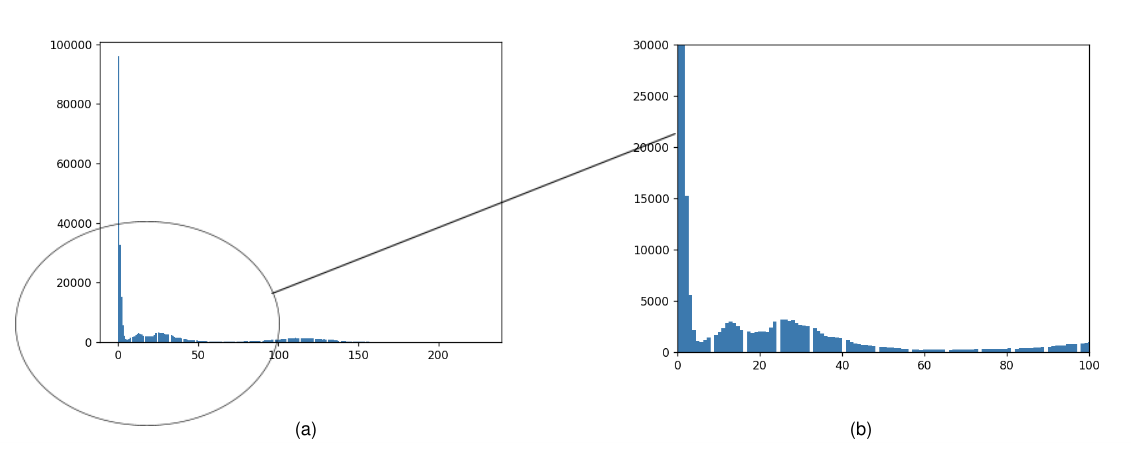
\includegraphics[scale=0.45]{bimodal_temple.jpg} 
\caption{Bimodal distribution of a  single temple image}
\label{fig:dist}
\end{figure}

In Figure \ref{fig:dist} (a), a histogram of the different intensities of pixels in a single image of the temple dataset is plotted. 
\\
The the x-axis just as in Figure \ref{fig:thresh}, refers to the different intensity values, with white being 255 and black being 0. The y-axis corresponds to the availability of the number of pixels at each intensity values of x-axis.
\\
Since out background is black and majority of the pixels in the image is black, high spike of over 95000 is seen at x = 0.
\\
Figure \ref{fig:dist} (b) is a zoomed in version to figure out the threshold value. It can be roughly estimated that from part(b) that the new spike would rise somewhere after 20. For our program, this has to be divided out of 255, to give us a threshold value among 0 to 1.
\newpage

The threshold value for all the 16 images of the temple dataset is taken and a mean is calculated:
\\
\begin{table}[h]
\begin{tabular}{lllllllllllllllll}
Image no (i): & 1 & 2 & 3 & 4 & 5  & 6 & 7 & 8 & 9 & 10 & 11 & 12 & 13 & 14 & 15 & 16\\
Threshold val (t): & 20 & 18 & 1 & 4 & 1 & 15 & 19 & 23 & 22 & 11 & 17 & 23 & 0 & 8 & 14 & 13 \\

\end{tabular}
\end{table}

Therefore the mean threshold:
\begin{equation}
mean = \frac{\sum \limits_{i=1}^{16} t^i}{16} = 13.0625
\end{equation}
Hence, the threshold calculated is:
\begin{equation}
threshold = \frac{13.0625}{255} = 0.0512
\end{equation}
\\
\subsection{Silhouettes of the temple dataset}
Silhouettes of the initial 16 images obtained by  running segmentation with threshold value of 0.0512:
\begin{figure}[h]
\includegraphics[scale=0.7]{silhouettes.jpg} 
\end{figure}
\newpage
\section{Transforming from 3D  world space to 2Dimage space}
\subsection{Camera Model}
\newpage

\subsection{Camera Matrix}

If you have a formal theorem you might try this.
\begin{definition}\label{def}
See definition~\ref{def}.
\end{definition}
\begin{theorem}
For all $n\in\nats,\; 1^n=1$.
\end{theorem}
\begin{proof}
By induction over $n$.
\end{proof}
\newpage

\chapter{Implementation}


\chapter{Conclusions}
\section{Achievements}
Summarise the achievements to confirm the project goals have been met.
\section{Evaluation}
Evaluation of the work (this may be in a separate chapter if there is substantial evaluation).

\section{Future Work}
How the project might be continued, but don't give the impression you ran out of time!

\appendix


\begin{thebibliography}{HHM99}


\bibitem[Pri70]{PriorNOP70}  %%only an example
A.~Prior.
\newblock The notion of the present.
\newblock {\em Studium Generale}, 23:  245--248, 1970.


\bibitem[Rey97]{Rey:D}
M.~Reynolds.
\newblock A decidable temporal logic of parallelism.
\newblock {\em Notre Dame Journal of Formal Logic}, 38(3):  419--436,
  1997.


\bibitem [Schneider 2014]{Schneider:2014}
David C. Schneider
\newblock  Shape from Silhouette
Computer Vision, 2014
ISBN : 978-0-387-30771-8



\bibitem[Cheung03]{Cheung:2003}
Kong Man German Cheung
\newblock    Visual Hull Construction, Alignment and Refinement for Human Kinematic Modeling, Motion Tracking and Rendering. 
\newblock PhD thesis, Carnegie Mellon University, 2003.

\bibitem [Roth82]{Roth:82}
Roth, S. D. 
\newblock “Ray Casting for Modeling Solids.” 
\newblock Computer Graphics and Image Processing, 18 (February 1982), 109-144.

\bibitem [Chen95]{Chen:95}
Chen, S. E. 
\newblock “Quicktime VR – An Image-Based Approach to Virtual
Environment Navigation.” SIGGRAPH 95

\bibitem [UoV2009]{UoV:09}
University of Victoria
\newblock https://www.ece.uvic.ca/~aalbu/computer\%20vision\%202009/Lecture\%209.\%20Segmentation-Thresholding.pdf

\bibitem[WWH]{WWH}
What When How
\newblock http://what-when-how.com/biomedical-image-analysis/intensity-based-segmentation-thresholding-biomedical-image-analysis/\#:\~:text=Biomedical\%20Image\%20Analysis)-,Intensity\%2DBased\%20Segmentation\%20(Thresholding)\%20(Biomedical\%20Image\%20Analysis),relevant\%20information\%20are\%20called\%20background.
\end{thebibliography}
\chapter{Other appendices, e.g., code listing}
Put your appendix sections here

\end{document}